% =============================================================================
% Multi-Camera VLM Reasoning Benchmark -- standalone, paste-ready Overleaf writeup
% Numbers reflect the VERIFIED analysis/ORIENTATION.md + why_models_fail.md
% (CVBench / CrossView project) as of 2026-06-22. Re-verify before submission.
%
% To use in Overleaf: paste this file (or merge sections into your existing doc)
% and upload the referenced figures (see \graphicspath / figure comments).
% Figures live in the repo at:
%   analysis/crossview_meva1033_out/accuracy_vs_orig_cameras.png  (camera curve, 1,033-Q)
%   analysis/crossview_meva1033_out/accuracy_by_task.png          (per-task accuracy)
%   analysis/reasoning_gain.png                                   (video uplift over blind)
% =============================================================================
\documentclass[11pt]{article}

\usepackage[margin=1in]{geometry}
\usepackage{booktabs}
\usepackage{graphicx}
\usepackage{amsmath}
\usepackage{xcolor}
\usepackage[hidelinks]{hyperref}
\usepackage{caption}

\graphicspath{{figures/}{../analysis/}{../analysis/crossview_meva1033_out/}}

\title{Benchmarking Vision--Language Models on Multi-Camera Reasoning:\\
       An Accuracy and Failure-Mode Analysis}
\author{ZEIOS Vanguards / CVBench multi-camera study}
\date{\today}

\begin{document}
\maketitle

\begin{abstract}
We study how vision--language models (VLMs) reason over \emph{multiple} synchronized (or
unrelated) camera views, and we read their failures off the models' own \texttt{<think>}
reasoning traces. Two benchmarks share one ``thinking'' evaluation harness: \textbf{CVBench/MVR}
(1--4 unrelated clips per question) and \textbf{CrossView} (2--4 synchronized views per question,
capped to $\le 4$), built from the MEVA surveillance and EgoExo4D datasets. We compare two
8B-parameter models, \textbf{Qwen3-VL-8B-Thinking} and \textbf{InternVL3-8B}. Our central finding
is that these benchmarks expose \emph{perception}, not reasoning: sparse 8-frame-per-clip sampling
almost never lands on the brief moment a queried event occurs, so the model is effectively shown a
still photo and asked a question about a movie. The cleanest evidence is a \emph{blind-beats-video}
inversion on CrossView (a text-only model scores 36.7\% vs.\ 31.7\% with
video). We characterize five failure modes, show accuracy degrades as the number of cameras rises,
and propose a multi-architecture, multi-metric benchmark (accuracy, latency, cost) to test whether
\emph{distributed} (per-stream) agents beat \emph{centralized} (single-VLM) ones per question
category.
\end{abstract}

\section{Introduction}
Multi-camera understanding---reasoning jointly over several synchronized video streams---is central
to surveillance, sports analytics, and embodied AI, yet it is essentially unbenchmarked for modern
VLMs. We ask a deceptively simple question: when a question requires integrating evidence across
cameras (relative motion, event ordering, cross-view correspondence), do today's VLMs actually
\emph{see} it, or do they fall back on language priors? We answer with interpretable
chain-of-thought traces rather than accuracy alone: accuracy is the means, the \texttt{<think>}
trace is the end.

\section{Benchmark setup}
\textbf{Datasets.} CrossView questions stack 2--4 clips from different cameras. We use two sources:
\emph{MEVA} (public surveillance, CC-BY, 100\% cap-answer-safe) and \emph{EgoExo4D}
(ego+exo views). A \emph{cap} of $\le 4$ clips is enforced; questions with more cameras are capped,
and a \texttt{cap\_answer\_safe} flag marks whether the gold answer survives the cap. \textbf{We
always stratify by this flag and never pool} MEVA (safe) with lossy-capped EgoExo4D.

\textbf{Models and harness.} Two legs share the schema: a Qwen leg
(\texttt{eval\_thinking.py}, HuggingFace transformers) and an InternVL leg (\texttt{lmms-eval}).
Both prompt for visible reasoning between \texttt{<think>...</think>} and a final choice between
\texttt{<answer>...</answer>}, and both sample \textbf{8 frames per clip}.

\textbf{Task families.} CrossView questions are \emph{Spatial} (how two people's distance evolves),
\emph{Temporal} (which event happened first), and \emph{Event-Ordering} (order 3--4 events
chronologically).

\section{Input pipeline (why ``8 frames'' matters)}
The two legs sample \emph{different} 8 frames, which matters because surveillance scenes are sparse.
Table~\ref{tab:sampling} contrasts them.

\begin{table}[h]
\centering
\caption{Frame-sampling asymmetry between the two legs (8 frames/clip each).}
\label{tab:sampling}
\begin{tabular}{lll}
\toprule
Mechanism & Qwen3-VL-8B-Thinking & InternVL3-8B \\
\midrule
Sampling formula & \texttt{linspace(0,\,total-1,\,8)} & segment midpoints \\
Endpoints        & \textbf{included} (frame 0 and last) & \textbf{excluded} \\
Per-video marker & text \texttt{"Video k:"} & pixel marker image \\
Vision tokens (4-video Q) & $\approx$\,11.5k & $\approx$\,10.3k \\
\bottomrule
\end{tabular}
\end{table}

On a $\sim$280\,s clip, both legs land four samples at roughly 21\,s, 107\,s, 193\,s, and 278\,s---
$\sim$85\,s apart. The queried person typically transits for only a few seconds, so the samples fall
\emph{between} events and every frame of a given camera looks identical. The models say so out loud:
across 1,033 traces the word ``static'' appears in \textbf{688}, ``no people / no movement'' in
\textbf{774}.

\section{Output parsing and a measurement fix}
The answer is taken from the \texttt{<answer>} tag; if absent (a truncated trace), parsing falls back
\emph{only} to an explicit ``the answer is X'' conclusion, otherwise it \textbf{abstains}
(returns the empty string, scored wrong but honest). This fixed a contamination artifact: an earlier
parser grabbed the first stray \texttt{A/B/C/D} token anywhere in the text (e.g.\ the article ``a''
in ``a vehicle''), fabricating a lucky letter on every truncated trace and making Event-Ordering a
mechanical \textbf{0/20}. After raising the token budget ($2048\!\rightarrow\!8192$) and hardening
the parser, Event-Ordering became a legitimate \textbf{7/20} (54/60 emit \texttt{<answer>},
3 abstain).

\section{Results}

\begin{table}[h]
\centering
\caption{Headline accuracies. Blind = text-only, no video.}
\label{tab:headline}
\begin{tabular}{llrrr}
\toprule
Benchmark & $n$ & Qwen3-VL (video) & Qwen3-VL (blind) & InternVL3 \\
\midrule
CVBench (45-Q)          & 45   & \textbf{62.2\%} & 40.0\% & 55.6\% \\
CrossView (60-Q)        & 60   & 31.7\%          & \textbf{36.7\%} & \textbf{38.3\%} \\
CrossView MEVA (1,033-Q)& 1033 & 30.9--32.0\%    & --     & \textbf{34.0\%} \\
\bottomrule
\end{tabular}
\end{table}

Two results stand out (Table~\ref{tab:headline}). First, on the \emph{real} CVBench benchmark video
genuinely helps (+22\,pp over blind). Second, on CrossView the direction \textbf{inverts}: a blind
model \emph{beats} the same model with video. Joining the paired 60-Q set by question id, 15
questions flip blind-RIGHT $\rightarrow$ video-WRONG vs.\ only 12 the other way; the net $+3$ exactly
equals the accuracy gap. Seeing uninformative frames actively overrides a correct prior-driven guess.

\paragraph{Per-task accuracy (1,033-Q).} The two models have nearly opposite strengths
(Table~\ref{tab:pertask}). The largest split is Temporal, where InternVL3 doubles Qwen.

\begin{table}[h]
\centering
\caption{Per-task accuracy on the 1,033-Q MEVA pool.}
\label{tab:pertask}
\begin{tabular}{lrr}
\toprule
Task ($n$) & Qwen3-VL & InternVL3 \\
\midrule
Spatial (431)        & 35\% (151) & 28\% (119) \\
Temporal (305)       & 25\% (75)  & \textbf{51\% (157)} \\
Event-Ordering (297) & 31\% (93)  & 25\% (75) \\
\bottomrule
\end{tabular}
\end{table}

The Temporal split is about \emph{commitment}, not perception: every Temporal question's gold answer
is A or B, but Qwen escapes to D (``cannot be determined,'' 142/305) or C (8/305)---all guaranteed
wrong---while InternVL commits to A/B in 292/305. When \emph{both} models commit to A/B their
accuracy is nearly identical (Qwen 49\% vs.\ InternVL 54\%), so Qwen's entire deficit is the
$\sim$150 questions it throws away on escape options.

\paragraph{Accuracy falls as cameras rise.} Accuracy degrades from \textbf{41\%} on 2-camera
questions to \textbf{25--26\%} at 12--14 cameras (Figure~\ref{fig:cameracurve})---more views, harder
correspondence, worse accuracy. This is the central ``multi-camera is hard'' thesis.

\begin{figure}[h]
\centering
% upload analysis/crossview_meva1033_out/accuracy_vs_orig_cameras.png to Overleaf
\fbox{\parbox{0.7\linewidth}{\centering\vspace{1.5cm}
\texttt{accuracy\_vs\_orig\_cameras.png}\\(accuracy vs.\ original camera count)\vspace{1.5cm}}}
% 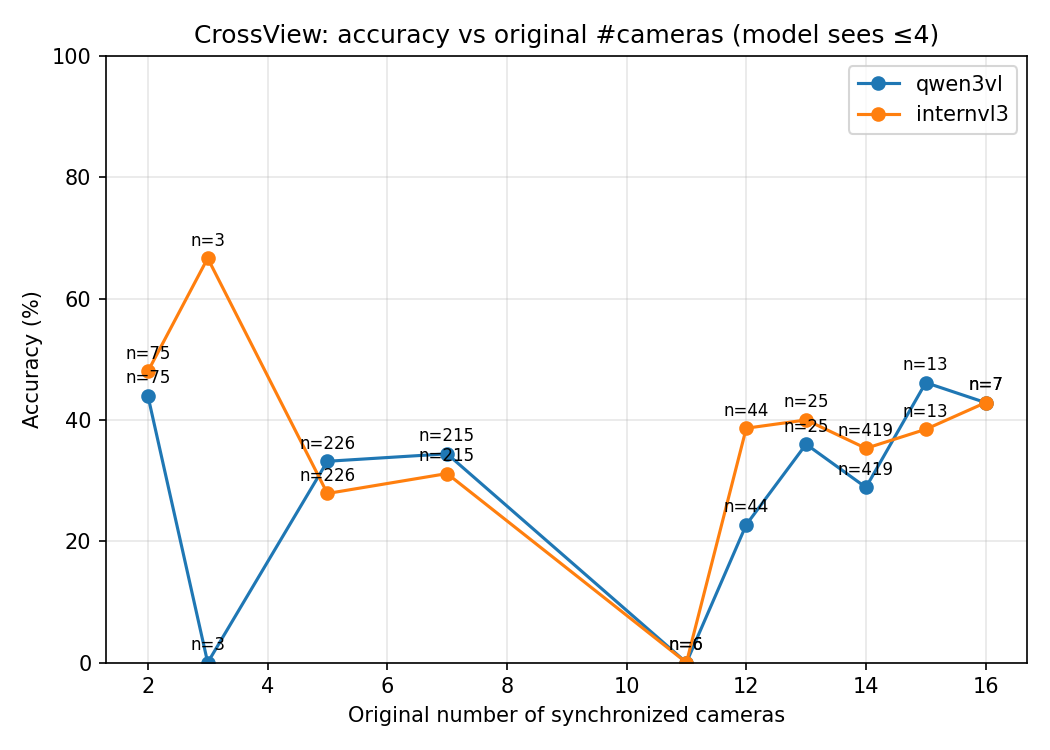
\includegraphics[width=0.7\linewidth]{accuracy_vs_orig_cameras.png}
\caption{Accuracy declines monotonically as the true (pre-cap) camera count rises.}
\label{fig:cameracurve}
\end{figure}

\section{Failure analysis}
The causal chain runs \emph{left to right}: sparse sampling $\rightarrow$ empty-looking frames
$\rightarrow$ failed grounding $\rightarrow$ prior-driven reasoning $\rightarrow$ wrong answer.
The reasoning is not the root cause; the missing input is. Table~\ref{tab:taxonomy} quantifies the
Qwen failure modes (of 714 wrong on the 1,033-Q pool).

\begin{table}[h]
\centering
\caption{Failure taxonomy, Qwen3-VL, 1,033-Q (of 714 wrong answers).}
\label{tab:taxonomy}
\begin{tabular}{lr l}
\toprule
Mode & Count & Note \\
\midrule
\texttt{wrong\_reasoned}       & 626 & reads emptied frames, reasons to the wrong conclusion \\
\texttt{truncation\_no\_answer}& 69  & 60 are Event-Ordering (long chains exhaust the budget) \\
\texttt{given\_order\_bias}    & 13  & all Event-Ordering \\
\texttt{single\_video\_shortcut}& 6  & all Spatial \\
\bottomrule
\end{tabular}
\end{table}

The dominant mode (\texttt{wrong\_reasoned}, 88\% of errors) is the model perceiving sparse frames as
static, then either hallucinating concrete scene contents to reason over, treating the arbitrary clip
numbering (``Video 1, 2, 3'') as a timeline, or misreading the printed per-frame sampling offsets
(21.4\,s, 107.1\,s, \dots) as wall-clock event times.

\section{Threats to validity}
(i) The contaminated early run (stray-letter parser on truncated traces) is archived and excluded;
all numbers use the abstain-safe parser. (ii) We stratify by \texttt{cap\_answer\_safe} and never pool
MEVA with lossy-capped EgoExo4D. (iii) An \texttt{analyze\_failures.py} re-parse recovers
$\sim$12 borderline answers (30.9\% $\rightarrow$ 32.0\% on the 1,033-Q Qwen run); failure-mechanism
\emph{proportions} are parser-insensitive.

\section{Proposed benchmark and next steps}
The failure analysis motivates a systems-level benchmark: compare \textbf{architectures}
(A0 centralized single-VLM; A1 distributed one-VLM-per-stream + aggregator; A2 router; A3 NeuS-QA)
on \textbf{multiple metrics} (accuracy, latency including a parallelizable estimate, token/compute
cost, abstention) across three open VLM backends. The key question---\emph{for which question
categories does a distributed agent beat a centralized one?}---follows directly from the
cross-view-correspondence failures documented above: we expect distribution to help Spatial
(independent per-camera grounding) but hurt Temporal/Event-Ordering (which need cross-stream
synchronization). Further directions include 2-camera temporal alignment before VLM ingestion, and
neural-reconstruction (NeuS) QA.

\section*{Reproducibility}
All numbers trace to files in the project \texttt{analysis/} directory: \texttt{ORIENTATION.md}
(results inventory, \S8), \texttt{why\_models\_fail.md} (failure taxonomy and per-task counts),
\texttt{input\_pipeline.md} (sampling), and \texttt{blind\_sanity.md} (the text-only baseline is
genuinely zero-vision-token).

\end{document}
